\subsection{Hillslope model (model ID: 13)}
The Hillslope model (fig.~\ref{fig:13_schematic}) is a conceptualization of the perceived dominant processes in a typical Western European hillslope \citep{Savenije2010}. It belongs to a 3-part topography driven modelling exercise, together with a wetland and plateau conceptualization. Each model is provided in isolation here, because they are well-suited for isolating specific model structure choices. It has 2 store and 7 parameters ($D_w$, $S_{h,max}$, $\beta_h$, $a$, $T_h$, $C$ and $K_h$). The model aims to represent:

\begin{itemizecompact}
\item Stylized interception by vegetation;
\item Evaporation;
\item Separation between rapid subsurface flow and groundwater recharge;
\item Capillary rise and linear relation runoff from groundwater.
\end{itemizecompact}

\subsubsection{File names}
\begin{tabular}{@{}ll}
Model: &m\_13\_hillslope\_7p\_2s \\
Parameter ranges: &m\_13\_hillslope\_7p\_2s\_parameter\_ ranges \\
\end{tabular}

% Equations
\subsubsection{Model equations}

% Model layout figure
{ 																	% This ensures it doesn't warp text further down
\begin{wrapfigure}{l}{7cm}
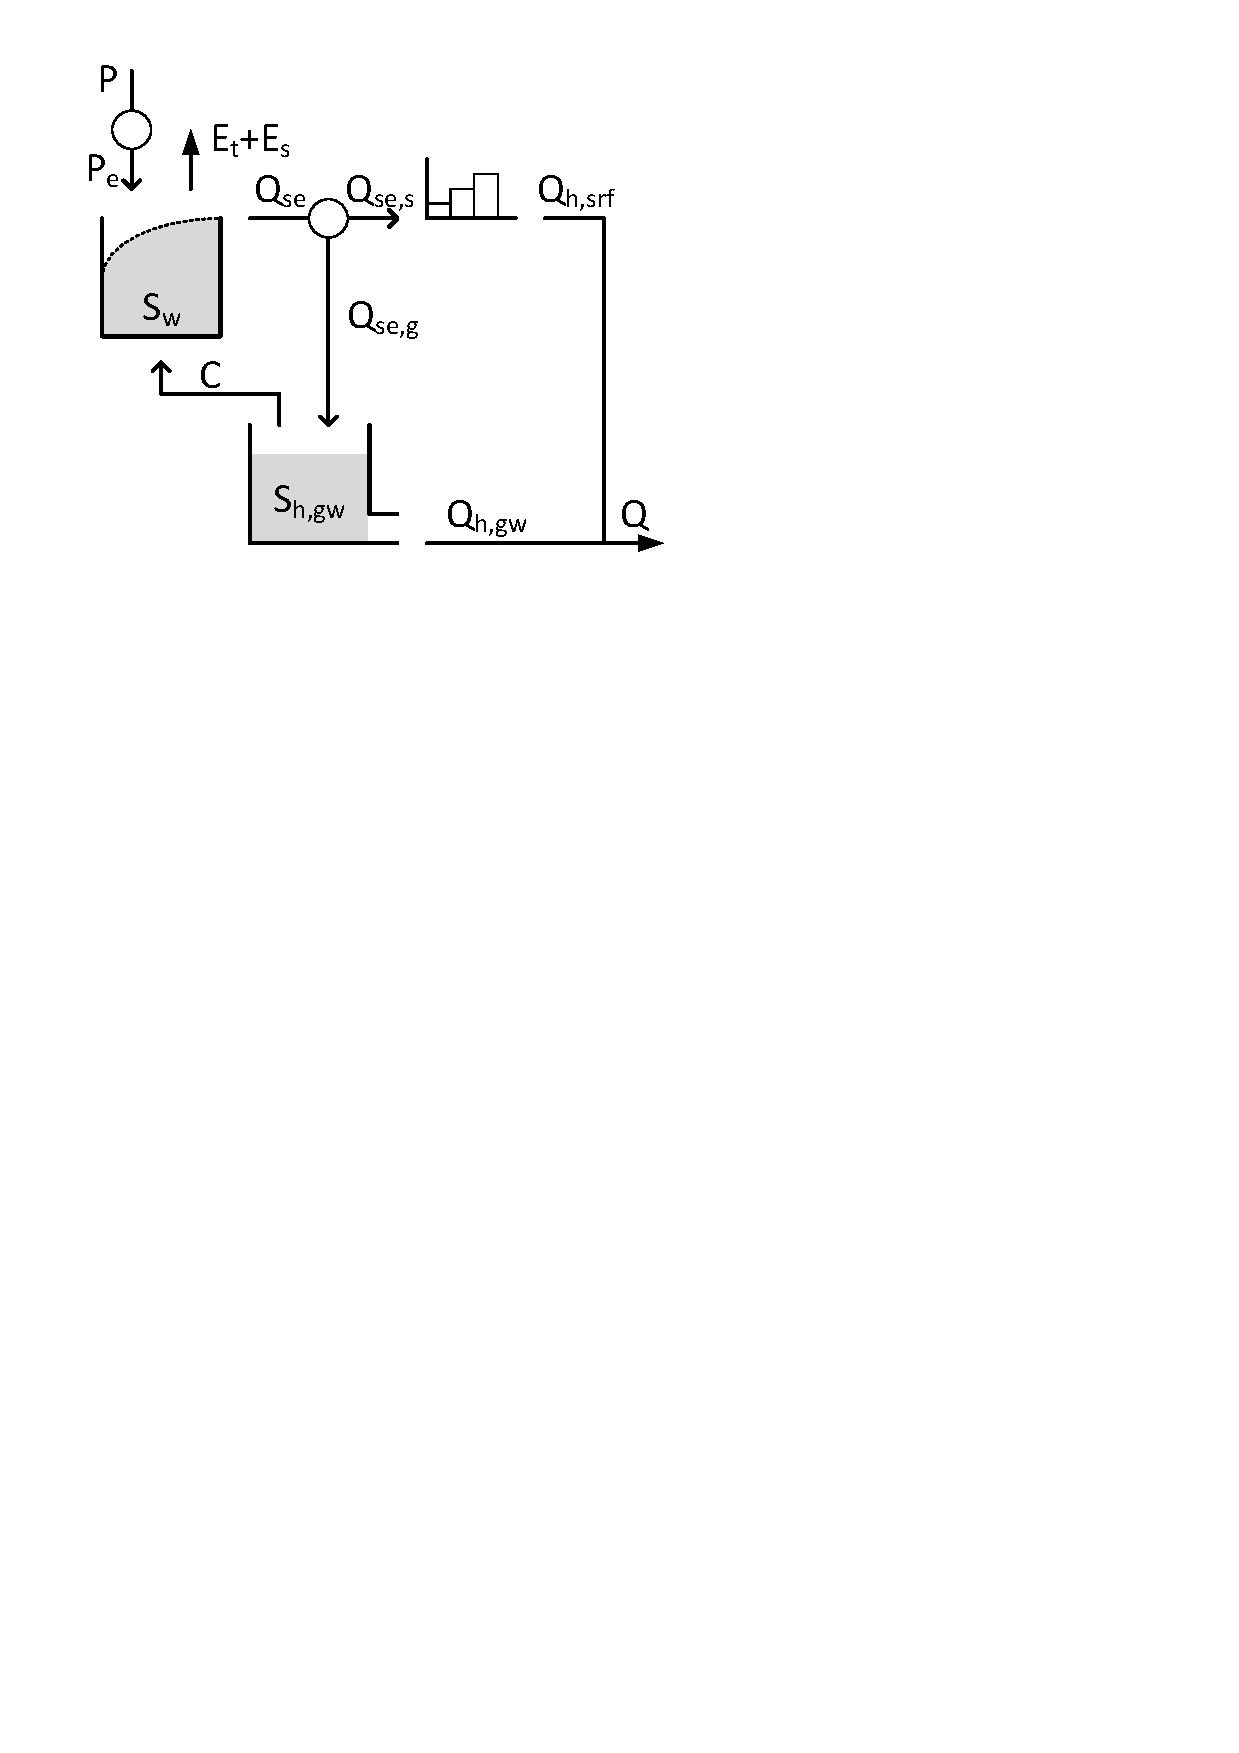
\includegraphics[trim=1cm 20.3cm 9cm 1cm,width=7cm,keepaspectratio]{./files/13_schematic.pdf}
\caption{Structure of the Hillslope model} \label{fig:13_schematic}
\end{wrapfigure}

\begin{align}
	\frac{dS_w}{dt} &= P_e+C-(E_t+E_s)-Q_{se} \\
	P_e &= max(P-D_h,0)\\
	C &= c.\\
	E_t+E_s &= 
	\begin{cases}
		E_p, & \text{if } S_w > 0 \\
		0, & \text{otherwise}\\
	\end{cases}\\
	Q_{se} &= \left(1-\left(1-\frac{S_h}{S_{h,max}}\right)^{\beta_h}\right)*P_e\\
\end{align}

Where $S_w$ is the current soil water storage [mm]. Incoming precipitation P [mm/d] is reduced by interception $D_h$ [mm/d], which is 

} % end of wrapfigure fix

assumed to evaporate before the next precipitation event. $C$ is capillary rise from groundwater [mm/d], given as a constant rate. Evaporation from soil moisture $E_t+E_s$ [mm/d] occurs at the potential rate $E_p$ whenever possible. Storage excess surface runoff $Q_{se}$ [mm/d] depends on the fraction of the catchment that is currently saturated, expressed through parameters $S_{h,max}$ [mm] and $\beta_h$ [-]. 

\begin{align}
	\frac{dS_{h,gw}}{dt} &= Q_{se,g}-C-Q_{h,gw} \\
	Q_{se,g} &= (1-a)*Q_{se}\\
	Q_{h,gw} &= K_h*S_{h,gw}
\end{align}

Where $S_{h,gw}$ is current groundwater storage [mm]. $Q_{se,g}$ is the groundwater fraction of storage excess flow $Q_{se}$ [mm/d], with $Q_{se,s}$ as its complementary part. $a$ is the parameter controlling this division [-]. Groundwater flow $Q_{h,gw}$ [mm/d] depends linearly on current storage $S_{h,gw}$ through parameter $K_h$ [$d^{-1}$]. Total flow $Q_t$ is the sum of $Q_{h,gw}$ and $Q_{h,srf}$, the latter of which is $Q_{se,s}$ lagged over $T_h$ days.

\subsubsection{Parameter overview}
% Table generated by Excel2LaTeX from sheet 'Sheet1'
\begin{table}[htbp]
  \centering
    \begin{tabular}{lll}
    \toprule
    Parameter & Unit  & Description \\
    \midrule
    $D_w$ & $mm~d^{-1}$ & Interception evaporation  \\
    $S_{h,max}$ & $mm$  & Maximum soil moisture storage \\
    $\beta_h$ & $-$   & Non-linearity parameter for contributing area \\
    $a$   & $-$   & Fraction saturation excess to groundwater \\
    $T_h$ & $d$   & Unit Hydrograph time base \\
    $C$   & $mm~d^{-1}$ & Capillary rise \\
    $K_h$ & $d^{-1}$ & Runoff coefficient \\
    \bottomrule
    \end{tabular}%
  \label{tab:addlabel}%
\end{table}%

